\documentclass[titlepage,a4paper]{article}

\usepackage{a4wide}
\usepackage[colorlinks=true,linkcolor=black,urlcolor=blue,bookmarksopen=true]{hyperref}
\usepackage{bookmark}
\usepackage{fancyhdr}
\usepackage[spanish]{babel}
\usepackage[utf8]{inputenc}
\usepackage[T1]{fontenc}
\usepackage{listings}
\usepackage{graphicx}
\usepackage{float}
\usepackage{hyperref}
\pagestyle{fancy} % Encabezado y pie de página
\fancyhf{}
\fancyhead[L]{Ejercicios de Parcial}
\fancyhead[R]{Introducción a Sistemas Distribuidos - FIUBA}
\renewcommand{\headrulewidth}{0.4pt}
\fancyfoot[C]{\thepage}
\renewcommand{\footrulewidth}{0.4pt}



% code listing settings
\usepackage{listings}
\renewcommand{\lstlistingname}{Código \textnumero{}}
\lstset{
    language=Python,
    basicstyle=\ttfamily\small,
    aboveskip={1.0\baselineskip},
    belowskip={1.0\baselineskip},
    columns=fixed,
    extendedchars=true,
    breaklines=true,
    tabsize=4,
    prebreak=\raisebox{0ex}[0ex][0ex]{\ensuremath{\hookleftarrow}},
    frame=lines,
    showtabs=false,
    showspaces=false,
    showstringspaces=false,
    keywordstyle=\color[rgb]{0.627,0.126,0.941},
    commentstyle=\color[rgb]{0.133,0.545,0.133},
    stringstyle=\color[rgb]{01,0,0},
    numbers=left,
    numberstyle=\small,
    stepnumber=1,
    numbersep=10pt,
    captionpos=t,
    escapeinside={\%*}{*)}
}


\begin{document}
\begin{titlepage} % Carátula
	\hfill
\includegraphics[width=6cm]{logofiuba.jpg}
    \centering
    \vfill
    \Huge \textbf{Ejercicios parcial}
    \vskip2cm
    \Large [?]  Introducción Sistemas Distribuidos\\
    Curso Hamelin \\ 
    Primer cuatrimestre de 2022 
    \vfill
    \begin{tabular}{ | l | l | } % Datos del alumno
      \hline
      VAZQUEZ LAREU, Román & 100815 \\ \hline
      

  	\end{tabular}
    \vfill
    \vfill
\end{titlepage}

\tableofcontents % Índice general
\newpage

\section{Calcular RTT}\label{sec:CalcularRTT}

\textbf{Tiempo de inserción}: tiempo que tarda el paquete en ser insertado en el enlace

$$t_{ins} = \frac{L}{R}$$ 

\begin{itemize}
    \item $L$: largo del paquete
    \item $R$: velocidad de serialización
\end{itemize}


\textbf{Tiempo de propagación}: Tiempo que demora el paquete en propagarse por el enlace de un router al próximo

$$t_{prop} = \frac{d}{c}$$

\begin{itemize}
    \item $d$: distancia entre extremos del enlace
    \item $c$: velocidad del medio
        \subitem Aire: $c = 3x10^8 \frac{m}{s}$
        \subitem Fibra, cobre,etc: $\frac{2}{3} c$ 
\end{itemize}


\textbf{Qué tiempo es más influyente?}
\begin{itemize}
    \item Distancias largas: $ t_{ins} <  t_{prop} $
    \item Distancias cortas: $ t_{ins} > t_{prop}$
\end{itemize}





\begin{figure}[H]
\centering
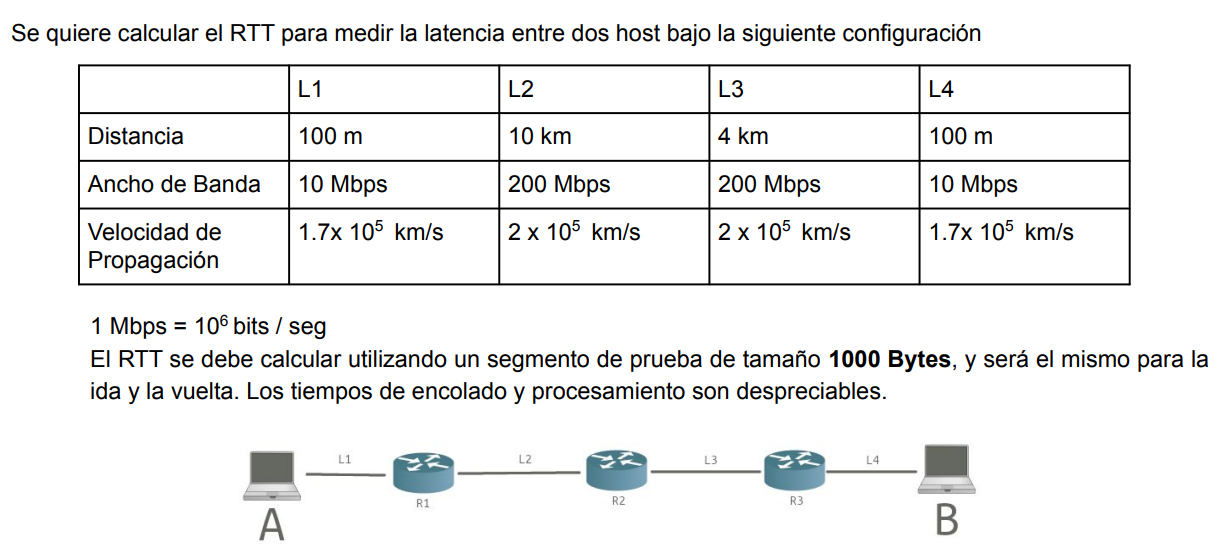
\includegraphics[width=\textwidth]{ejercicioRtt.png}
\end{figure}


RTT o Round-Trip-Time es el tiempo que tarda un paquete de datos enviado desde un emisor en volver
al mismo emisor habiendo pasado por el receptor de destino.

Al tener las velocidades de propagación en $\frac{Km}{s}$, se pasan las distancias a $Km$

$$D_{L1} = 100 m = 0.1 \; Km$$
$$D_{L2} = 10 \; Km$$
$$D_{L3} = 4 \; Km$$
$$D_{L4} = 100 m = 0.1 \; Km$$

Se pasa el ancho de banda a $bits/seg$

$$t_{ins1} = 10 Mbps = 10^7 \frac{bits}{seg}$$
$$t_{ins2} = 200 Mbps = 20\cdot 10^7 \frac{bits}{seg}$$
$$t_{ins3} = 200 Mbps = 20\cdot 10^7 \frac{bits}{seg}$$
$$t_{ins4} = 10 Mbps = 10^7 \frac{bits}{seg}$$

Largo del paquete a $bits$

$$1000 \; bytes = 8000 \; bits$$

\textbf{Análisis tiempo de inserción}: \\


\begin{figure}[H]
\centering
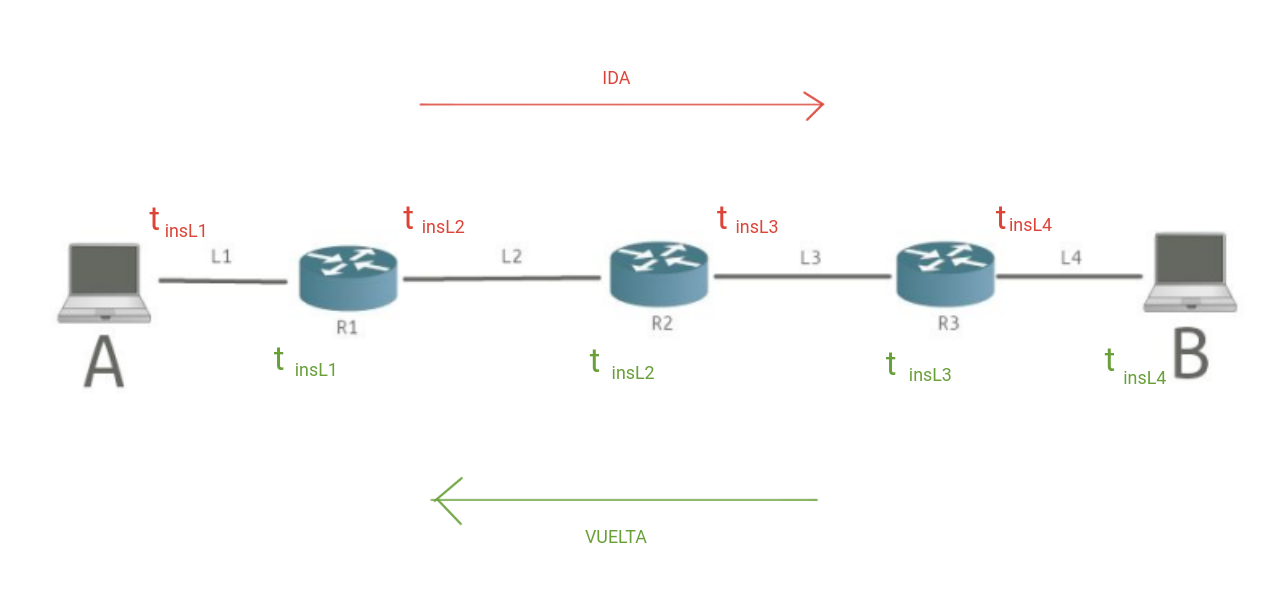
\includegraphics[width=\textwidth]{tiempoInsercion.png}
\end{figure}



Ida:

$$ t_{insIDA} = t_{insL1} + t_{insL2} + t_{insL3} +t_{insL4} $$ 
$$\frac{8000 bits}{10^7 \frac{bits}{seg}}  + \frac{8000 bits}{20\cdot 10^7 \frac{bits}{seg}}  + \frac{8000 bits}{20\cdot 10^7 \frac{bits}{seg}} + \frac{8000 bits}{10^7 \frac{bits}{seg}} = 1.68 \cdot 10^-3 seg$$

Vuelta:

$$ t_{insVUELTA} = t_{insL4} + t_{insL3} + t_{insL2} +t_{insL1} $$ 
$$  \frac{8000 bits}{10^7 \frac{bits}{seg}}  + \frac{8000 bits}{20\cdot 10^7 \frac{bits}{seg}}  + \frac{8000 bits}{20\cdot 10^7 \frac{bits}{seg}} + \frac{8000 bits}{10^7 \frac{bits}{seg}} = 1.68 \cdot 10^{-3} seg $$

Total:

$$ t_{ins} = t_{insIDA} + t_{insVUELTA} =   1.68 \cdot 10^{-3} seg +  1.68 \cdot 10^{-3} seg =  3.36 \cdot 10^{-3} \; seg$$


\textbf{Análisis tiempo de propagación}: \\

\begin{figure}[H]
\centering
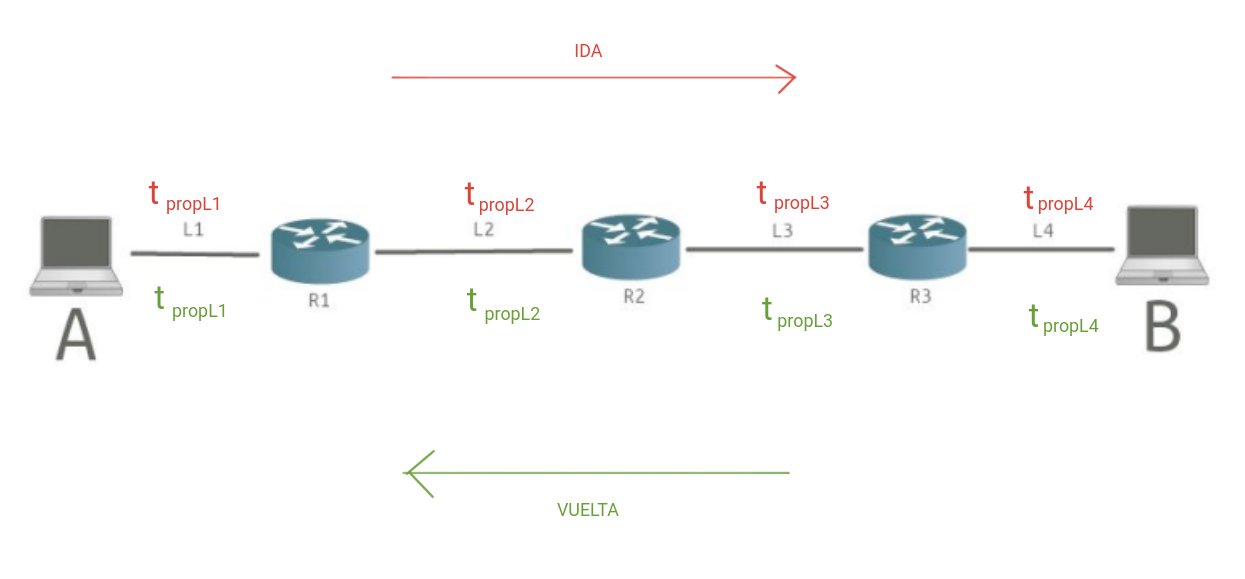
\includegraphics[width=\textwidth]{tiempoPropagacion.png}
\end{figure}

Ida:

$$t_{propIDA} = t_{propL1} + t_{propL2}  + t_{propL3} + t_{propL4} $$ 
$$ \frac{0.1 \; Km}{1.7\cdot10^5\frac{Km}{seg}} + \frac{10 \; Km}{2\cdot10^5\frac{Km}{seg}} + \frac{4 \; Km}{2\cdot10^5\frac{Km}{seg}} + \frac{0.1 \; Km}{1.7\cdot10^5\frac{Km}{seg}} = 7.11765 \cdot 10^{-5} \; seg $$

Vuelta:

$$t_{propVUELTA} = t_{propL4} + t_{propL3} + t_{propL2} + t_{propL1} $$ 
$$ \frac{0.1 \; Km}{1.7\cdot10^5\frac{Km}{seg}} + \frac{10 \; Km}{2\cdot10^5\frac{Km}{seg}} + \frac{4 \; Km}{2\cdot10^5\frac{Km}{seg}} + \frac{0.1 \; Km}{1.7\cdot10^5\frac{Km}{seg}} = 7.11765 \cdot 10^{-5} \; seg  $$

Total:

$$t_{prop} = t_{propIDA} + t_{propVUELTA}  =  7.11765 \cdot 10^{-5} \; seg + 7.11765 \cdot 10^{-5} \; seg = 1.42353\cdot10^{-4} \; seg$$

\textbf{Resolución final}:

$$ t_{prop} + t_{ins} = 1.42353\cdot10^{-4} \; seg + 3.36 \cdot 10^{-3} \; seg = 3.50235 \cdot 10^{-3} \; seg$$


\subsection{Otros}

\textbf{Tiempo de procesamiento}: es el tiempo que requiere el procesamiento del paquete en los routers. Implica leer el header y tomar la decisión de por cuál enlace enviarlo. Los órdenes de tiempo se encuentran entre los nano y microsegundos ($ns$, $\mu s$ )

\textbf{Tiempo de encolado}: es el tiempo que espera paquete en el router desde que arriba hasta que es finalmente transmitido. Depende de la tasa de desocupación del router, del tamaño de la cola. A mayor tráfico, mayor tiempo encolado. Este tiempo no es constante sino aleatorio, varía con el tráfico

\begin{figure}[H]
\centering
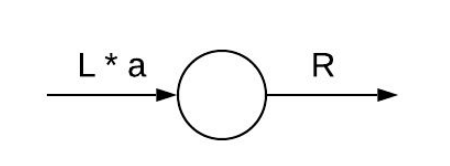
\includegraphics[width=\textwidth]{tiempoEncolado.png}
\caption{Tiempo de Encolado}
\end{figure}

\begin{itemize}
    \item L: largo del paquete
    \item a: tasa de arribo promedio de paquete
    \item R: velocidad de serialización
\end{itemize}

Si $L \cdot a > R$, significa que están llegando más paquetes que los que el router puede procesar, se va llenando el buffer hasta estarlo por completo y comenzar a descartar paquetes. Si $L \cdot a = R$ la cola se llena, entonces la solución es la subutilización, es decir $L \cdot a < R$

\begin{figure}[H]
\centering
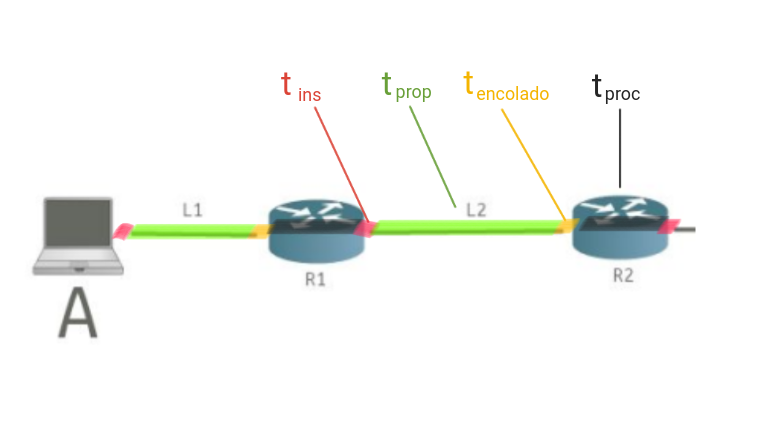
\includegraphics[width=\textwidth]{tiemposRTT.png}
\caption{Tiempo de Encolado}
\end{figure}

\section{Agregación de prefijos}\label{sec:agrprefijos}

Permite reducir la cantidad de entradas en la tabla de ruteo. Puede realizarse cuando \textbf{las redes son contiguas} y cuando tienen \textbf{idéntico Next Hop o puerto de salida}. Se dice que dos redes son contiguas cuando tienen \textbf{prefijos de igual longitud} y \textbf{la máscara sólo difiere en el último bit}


\subsection{Caso Favorable}

\begin{center}
    \begin{tabular}{c|c}
        Máscara & Puerto de salida \\
        \hline
        \hline
         192.168.0.0/24 &  0\\
         \hline
         192.168.1.0/24 &  0
    \end{tabular}
\end{center}

El \textbf{/24} indica que deben tomarse los primeros 24 bits
Si pasamos a binario:

\begin{center}
    \begin{tabular}{c|c|c|c}
        0-7 bits & 8-14 bits & 15-23 bits & 24-31 bits \\
        \hline
        \hline
        192 & 168 & 0000000 \textbf{0} & 00000000 \\
        \hline
        192 & 168 & 0000000 \textbf{1} & 00000000 \\
    \end{tabular}
\end{center}

Difieren sólo en el último bit (el bit número 24) y el prefijo es de igual longitud, por lo que son contiguas. Además tienen el mismo puerto de salida. Se puede hacer agregación de prefijos

\begin{center}
    \begin{tabular}{c|c}
        Máscara & Puerto de salida \\
        \hline
        \hline
         192.168.0.\textbf{0/23} &  0\\
    \end{tabular}
\end{center}

Se disminuyó en uno la máscara y se las unificó en una sola red

\subsection{Caso Desfavorable por no ser contiguas - bit}

\begin{center}
    \begin{tabular}{c|c}
        Máscara & Puerto de salida \\
        \hline
        \hline
         192.168.1.0/24 &  0\\
         \hline
         192.168.2.0/24 &  0
    \end{tabular}
\end{center}

El \textbf{/24} indica que deben tomarse los primeros 24 bits
Si pasamos a binario:

\begin{center}
    \begin{tabular}{c|c|c|c}
        0-7 bits & 8-14 bits & 15-23 bits & 24-31 bits \\
        \hline
        \hline
        192 & 168 & 000000 \textbf{01} & 00000000 \\
        \hline
        192 & 168 & 000000 \textbf{10} & 00000000 \\
    \end{tabular}
\end{center}

No difieren únicamente en el último bit, por lo que no cumplen con ser contiguas, por lo que no se puede realizar agregación de prefijos


\subsection{Caso Desfavorable por no ser contiguas - Next Hop}

\begin{center}
    \begin{tabular}{c|c}
        Máscara & Puerto de salida \\
        \hline
        \hline
         192.168.0.0/24 &  \textbf{0}\\
         \hline
         192.168.1.0/24 &  \textbf{1}
    \end{tabular}
\end{center}

Si bien son contiguas, al no compartir el next hop, no se puede realizar agregación de prefijos


\subsection{Ejercicio de parcial}

Simplificar la siguiente tabla

\begin{center}
    \begin{tabular}{c|c}
        Máscara & Puerto de salida \\
        \hline
        \hline
        157.128.2.0/23 &  0\\
        \hline
        168.123.0.0/24 &  1 \\
        \hline
        168.123.1.0/24 &  1 \\
        \hline
        168.12.128.0/19 &  2 \\
        \hline
        168.12.160.0/19 &  2 \\
    \end{tabular}
\end{center}


Únicamente se podrá hacer agregación en aquellas que tengan igual puerto de salida, serán las que se analizarán.
Se analizan las del puerto de salida 1

\begin{center}
    
    \begin{tabular}{c|c|c|c}

        0-7 bits & 8-14 bits & 15-23 bits & 24-31 bits \\
        \hline
        \hline
        168 & 123 & 0000000 \textbf{0} & 00000000 \\
        \hline
        168 & 123 & 0000000 \textbf{1} & 00000000 \\
    \end{tabular}
\end{center}


Difieren en el último bit, el prefijo es de igual longitud y el mismo puerto de salida. Realizo agregación de prefijos.


\begin{center}
    \begin{tabular}{c|c}
        Máscara & Puerto de salida \\
        \hline
        \hline
        168.123.0.0/23 &  1 \\
    \end{tabular}
\end{center}

Se analizan las del puerto de salida 2

\begin{center}
    \begin{tabular}{c|c|c|c}
        0-7 bits & 8-14 bits & 15-23 bits & 24-31 bits \\
        \hline
        \hline
        168 & 12 & 10\textbf{0} 00001 & 00000000 \\
        \hline
        168 & 12 & 10\textbf{1} 00000 & 00000000 \\
    \end{tabular}
\end{center}

Difieren en el último bit, el prefijo es de igual longitud y el mismo puerto de salida. Realizo agregación de prefijos 

\begin{center}
    \begin{tabular}{c|c}
        Máscara & Puerto de salida \\
        \hline
        \hline
        168.12.128.0/18 &  2 \\
    \end{tabular}
\end{center}

Tabla final simplificada

\begin{center}
    \begin{tabular}{c|c}
        Máscara & Puerto de salida \\
        \hline
        \hline
        157.128.2.0/23 &  0\\
        168.123.0.0/23 &  1 \\
        168.12.128.0/18 &  2 \\
    \end{tabular}
\end{center}

\section{Teoría}\label{sec:teoria}

\subsection{Protocolo\label{sec:protocolo}}


\subsubsection{ ¿Cuál es la función de un protocolo de capa de aplicación?}

La función de un protocolo de la capa de aplicación es la de ...

\subsubsection{¿Qué define un protocolo?} 


Un protocolo define:

\begin{itemize}
    \item Mensajes de petición y respuesta
    \item Sintaxis de los mensajes
    \item Campos - función, tamaño y delimitadores
    \item Procedimiento de envío de mensajes y sus respuestas
\end{itemize}


\end{document}
